%%%%%%%%%%%%%%
%% Run LaTeX on this file several times to get Table of Contents,
%% cross-references, and citations.

%% If you have font problems, you may edit the w-bookps.sty file
%% to customize the font names to match those on your system.

%% w-bksamp.tex. Current Version: Feb 16, 2012
%%%%%%%%%%%%%%%%%%%%%%%%%%%%%%%%%%%%%%%%%%%%%%%%%%%%%%%%%%%%%%%%
%
%  Sample file for
%  Wiley Book Style, Design No.: SD 001B, 7x10
%  Wiley Book Style, Design No.: SD 004B, 6x9
%
%
%  Prepared by Amy Hendrickson, TeXnology Inc.
%  http://www.texnology.com
%%%%%%%%%%%%%%%%%%%%%%%%%%%%%%%%%%%%%%%%%%%%%%%%%%%%%%%%%%%%%%%%

%%%%%%%%%%%%%
% 7x10
%\documentclass{wileySev}

% 6x9
\documentclass{wileySix}

\usepackage{graphicx}
\usepackage{listings}

\usepackage{color}
 
\definecolor{codegreen}{rgb}{0,0.6,0}
\definecolor{codegray}{rgb}{0.5,0.5,0.5}
\definecolor{codepurple}{rgb}{0.58,0,0.82}
\definecolor{backcolour}{rgb}{0.95,0.95,0.92}
 
\lstdefinestyle{mystyle}{
    backgroundcolor=\color{backcolour},   
    commentstyle=\color{codegreen},
    keywordstyle=\color{magenta},
    numberstyle=\tiny\color{codegray},
    stringstyle=\color{codepurple},
    basicstyle=\footnotesize,
    breakatwhitespace=false,         
    breaklines=true,                 
    captionpos=b,                    
    keepspaces=true,                 
    numbers=left,                    
    numbersep=5pt,                  
    showspaces=false,                
    showstringspaces=false,
    showtabs=false,                  
    tabsize=2,
    language=sh
}
 
\lstset{style=mystyle}

%%%%%%%
%% for times math: However, this package disables bold math (!)
%% \mathbf{x} will still work, but you will not have bold math
%% in section heads or chapter titles. If you don't use math
%% in those environments, mathptmx might be a good choice.

% \usepackage{mathptmx}

% For PostScript text
\usepackage{w-bookps}

%%%%%%%%%%%%%%%%%%%%%%%%%%%%%%%%%%%%%%%%%%%%%%%%%%%%%%%%%%%%%%%%
%% Other packages you might want to use:

% for chapter bibliography made with BibTeX
% \usepackage{chapterbib}

% for multiple indices
% \usepackage{multind}

% for answers to problems
% \usepackage{answers}

%%%%%%%%%%%%%%%%%%%%%%%%%%%%%%
%% Change options here if you want:
%%
%% How many levels of section head would you like numbered?
%% 0= no section numbers, 1= section, 2= subsection, 3= subsubsection
%%==>>
\setcounter{secnumdepth}{3}

%% How many levels of section head would you like to appear in the
%% Table of Contents?
%% 0= chapter titles, 1= section titles, 2= subsection titles, 
%% 3= subsubsection titles.
%%==>>
\setcounter{tocdepth}{2}

%% Cropmarks? good for final page makeup
%% \docropmarks

%%%%%%%%%%%%%%%%%%%%%%%%%%%%%%
%
% DRAFT
%
% Uncomment to get double spacing between lines, current date and time
% printed at bottom of page.
% \draft
% (If you want to keep tables from becoming double spaced also uncomment
% this):
% \renewcommand{\arraystretch}{0.6}
%%%%%%%%%%%%%%%%%%%%%%%%%%%%%%

%%%%%%% Demo of section head containing sample macro:
%% To get a macro to expand correctly in a section head, with upper and
%% lower case math, put the definition and set the box 
%% before \begin{document}, so that when it appears in the 
%% table of contents it will also work:

\newcommand{\VT}[1]{\ensuremath{{V_{T#1}}}}

%% use a box to expand the macro before we put it into the section head:

\newbox\sectsavebox
\setbox\sectsavebox=\hbox{\boldmath\VT{xyz}}

%%%%%%%%%%%%%%%%% End Demo


\begin{document}


\booktitle{Panduan Cerdas Mengenal Aplikasi Bank Sampah}
\subtitle{Berbasis Web serta terdapat UI Android}

\authors{Arrizal Furqona Gifary dan Bakti Qilan Mufid\\
\affil{Informatics Research Center}
%Floyd J. Fowler, Jr.\\
%\affil{University of New Mexico}
}

\offprintinfo{Panduan Cerdas Mengenal Aplikasi Bank Sampah}{Arrizal Furqona Gifary dan Bakti Qilan Mufid}
%% Can use \\ if title, and edition are too wide, ie,
%% \offprintinfo{Survey Methodology,\\ Second Edition}{Robert M. Groves}

%%%%%%%%%%%%%%%%%%%%%%%%%%%%%%
%% 
\halftitlepage

\titlepage


\begin{copyrightpage}{2019}
%Survey Methodology / Robert M. Groves . . . [et al.].
%\       p. cm.---(Wiley series in survey methodology)
%\    ``Wiley-Interscience."
%\    Includes bibliographical references and index.
%\    ISBN 0-471-48348-6 (pbk.)
%\    1. Surveys---Methodology.  2. Social 
%\  sciences---Research---Statistical methods.  I. Groves, Robert M.  II. %
%Series.\\
%
%HA31.2.S873 2007
%001.4'33---dc22                                             2004044064
\end{copyrightpage}

\dedication{`Jika Kamu tidak dapat menahan lelahnya belajar, 
Maka kamu harus sanggup menahan perihnya Kebodohan.'
~Imam Syafi'i~}

\begin{contributors}
\name{Nisa Hanum Harani, S.Kom., M.T.} D4 Teknik Informatika, Politeknik Pos Indonesia, Bandung,
Indonesia
\name{Arriza Furqona Gifary,} D4 Teknik Informatika, Politeknik Pos Indonesia, Bandung,
Indonesia
\name{Bakti Qilan Mufid,} D4 Teknik Informatika, Politeknik Pos Indonesia, Bandung,
Indonesia
\end{contributors}

\contentsinbrief
\tableofcontents
\listoffigures
\listoftables
\lstlistoflistings


\begin{foreword}
Sepatah kata dari Kaprodi, Kabag Kemahasiswaan dan Mahasiswa
\end{foreword}

\begin{preface}
Buku ini diciptakan sebagai produk hasil dari matakuliah proyek III dan sebagai peningkatan kemampuan mahasiswa.

\prefaceauthor{Penulis}
\where{Bandung, Jawa Barat\\
Februari, 2020}
\end{preface}


\begin{acknowledgments}
Terima kasih atas semua masukan dari para mahasiswa agar bisa membuat buku ini 
lebih baik dan lebih mudah dimengerti.

Terima kasih ini juga ditujukan khusus untuk team IRC yang 
telah fokus untuk belajar dan memahami bagaimana buku ini mendampingi proses 
Intership.
\authorinitials{R. M. A.}
\end{acknowledgments}

\begin{acronyms}
\acro{ACGIH}{American Conference of Governmental Industrial Hygienists}
\acro{AEC}{Atomic Energy Commission}
\acro{OSHA}{Occupational Health and Safety Commission}
\acro{SAMA}{Scientific Apparatus Makers Association}
\end{acronyms}

\begin{glossary}
\term{git}Merupakan manajemen sumber kode yang dibuat oleh linus torvald.

\term{bash}Merupakan bahasa sistem operasi berbasiskan *NIX.

\term{linux}Sistem operasi berbasis sumber kode terbuka yang dibuat oleh Linus Torvald
\end{glossary}

\begin{symbols}
\term{A}Amplitude

\term{\hbox{\&}}Propositional logic symbol 

\term{a}Filter Coefficient

\bigskip

\term{\mathcal{B}}Number of Beats
\end{symbols}

\begin{introduction}

%% optional, but if you want to list author:

\introauthor{Rolly Maulana Awangga, S.T., M.T.}
{Informatics Research Center\\
Bandung, Jawa Barat, Indonesia}

Pada era disruptif  \index{disruptif}\index{disruptif!modern} 
saat ini. git merupakan sebuah kebutuhan dalam sebuah organisasi pengembangan perangkat lunak.
Buku ini diharapkan bisa menjadi penghantar para programmer, analis, IT Operation dan Project Manajer.
Dalam melakukan implementasi git pada diri dan organisasinya.

Rumusnya cuman sebagai contoh aja biar keren\cite{awangga2018sampeu}.

\begin{equation}
ABC {\cal DEF} \alpha\beta\Gamma\Delta\sum^{abc}_{def}
\end{equation}

\end{introduction}

%%%%%%%%%%%%%%%%%%Isi Buku_

\chapter{Pengenalan}
\section{Pengenalan Bank Sampah}
Bank sampah ialah suatu terobosan yang berfokus pada pengelolaan sampah rumah tangga. Dimana sampah rumah tangga tersebut mampu di kelola dan memiliki timbal balik yang menguntungkan baik bagi rumah tangga yang mengeluarkan sampah, maupun pemerintah atau pengelola sampah. dengan hadirnya terobosan bank sampah ini diharapkan sampah-sampah rumah tangga dapat menguntungkan berbagai pihak. 

\chapter{Judul Bagian Kedua}
\section{Pengenalan}
\subsection{Sistem}
	\begin{figure}[H]
		
\includegraphics[width=6cm]{figures/web/php.png}
		\centering
		\caption{Logo PHP}
	\end{figure}
Sistem adalah suatu kelompok dari komponen-komponen yang saling berhubungan dengan satu sama lain dengan tujuan yang sama untuk mencapai tujuan tertentu. Sedangkan informasi adalah berupa data yang diolah menjadi bentuk lebih berguna dan berarti bagi pemakainya. Sehingga dapat disimpulkan bahwa system informasi adalah suatu komponen yang saling berhubungan yang bertujuan mengumpulkan,mengubah, dan menyebarkan informasi dalam sebuah organisasi.

Sistem terdiri dari bagian-bagian yang saling berkaitan yang beroperasi bersama untuk mencapai beberapa sasaran atau maksud (Budi Sutedjo, 2006:11 ). Sistem terdiri dari elemen-elemen yang berinteraksi untuk mencapai tujuan tertentu suatu sistem mempunyai karakteristik atau sifat-sifat tertentu. Terdapat dua kelompok pendekatan dalam mendefinisikan sistem, yaitu yang menekankan pada prosedurnya dan yang menekankan pada komponen atau elemennya. 
Suatu sistem adalah suatu jaringan kerja untuk melakukan suatu kegiatan atau untuk menyelesaikan suatu sasaran tertentu. Sedangkan pengertian prosedur itu sendiri menurut Richard F. Neuschel, prosedur suatu urutan operasi klerikal (tulis menulis), biasanya melibatkan beberapa orang dalam satu atau lebih departemen, yang diterapkan untuk menjamin penanganan yang seragam dari transaksi-transaksi bisnis yang terjadi.

\subsubsection{Karakteristik Sistem}
\hfill\\
Suatu sistem memiliki karakteristik atau sifat-sifat tertentu, yaitu (Sutabri, 2004:12): 153
\begin{enumerate}
	\item Komponen-komponen (\textit{Components})
	
Suatu sistem terdiri dari sejumlah komponen yang sering disebut dengan subsistem yang saling berinteraksi, yang artinya saling bekerja sama membentuk satu kesatuan. Komponen-komponen sistem atau elemen-elemen sistem dapat berupa suatu subsistem atau bagian-bagian dari sistem. Setiap subsistem mempunyai sifat-sifat dari sistem untuk menjalankan suatu fungsi tertentu dan mempengaruhi proses sistem secara keseluruhan.

	\item Batas sistem (Boundary) 

Batas sistem merupakan daerah yang membatasi antara suatu sistem dengan sistem yang lainnya atau dengan lingkungan luarnya. Batas sistem ini memungkinkan suatu sistem dipandang sebagai satu kesatuan. Batas suatu sistem menunjukkan ruang lingkup (scope) sistem itu sendiri. 

	\item Lingkungan luar sistem (Environments)
	
Lingkungan luar dari suatu sistem adalah apapun diluar batas dari sistem yang mempengaruhi operasi sistem. Lingkungan luar sistem dapat bersifat menguntungkan dan dapat juga bersifat merugikan sistem tersebut. 

	\item Penghubung sistem (Interface)
	 
Penghubung merupakan media penghubung antara subsistem dengan subsistem lainnya. Melalui penghubung ini memungkinkan sumber-sumber daya mengalir dari satu subsistem ke subsistem yang lainnya.
	
	\item Masukan sistem (Input)
	 
Masukan yaitu energi yang dimasukan ke dalam sistem, dimana dapat berupa masukan perawatan (maintenance input) dan masukan sinyal (signal input). Masukkan perawatan adalah energi yang di inputkan supaya sistem tersebut dapat beroperasi, sedang masukan sinyal adalah energi yang diproses untuk didapatkan keluaran.

	\item Keluaran sistem (Output)
	
Keluaran yaitu hasil dari energi yang diolah dan diklasifikasikan menjadi keluaran yang berguna dan sisa pembuangan.

	\item Pengolah sistem
	
Suatu sistem dapat mempunyai suatu bagian pengolah yang akan merubah input menjadi output.
	
	\item Sasaran sistem (Objective)
	
Suatu sistem pasti mempunyai tujuan (goal) atau sasaran (objective). Apabila suatu sistem tidak mempunyai sasaran, maka operasi sistem tidak ada gunanya.
\end{enumerate}

\subsubsection{Klasifikasi Sistem}
\hfill\\
Sistem dapat diklasifikasikan dari berbagai sudut pandang, diantaranya adalah sebagai berikut (Sutabri, 2004:14):

\begin{enumerate}
	\item Sistem abstrak dan sistem fisik. 
	
	Sistem abstrak adalah suatu sistem yang berupa ide-ide pemikiran atau ide-ide yang tidak tampak secara fisik, misalnya teologi yaitu sistem yang berupa pemikiran-pemikiran hubungan antara manusia dengan Tuhan.
Sedangkan sistem fisik adalah suatu sistem yang berupa pemikiran atau ide-ide yang nyata atau yang ada secara fisik. Misalnya sistem komputer, sistem akuntansi, sistem produksi dan lain sebagainya.

	\item Sistem alamiah dan sistem buatan manusia

	Sistem alamiah adalah sistem yang terjadi melalui proses alam, tidak dibuat manusia. Misalnya: sistem perputaran bumi. Sistem buatan manusia yang melibatkan interaksi antara manusia dengan mesin disebut dengan human-machine system atau ada yang menyebut dengan man-machine system.

	\item Sistem tertentu dan sistem tak tentu

	Sistem tertentu beroperasi dengan tingkah laku yang sudah dapat diprediksi. Contohnya: sistem komputer. Sistem tak tentu adalah sistem yang kondisi  masa depannya tidak dapat diprediksi karena mengandung unsur probabilitas.

	\item Sistem tertutup dan sistem terbuka
	Sistem tertutup merupakan sistem yang tidak berhubungan dan tidak berpengaruh dengan lingkungan luarnya. Sedangkan sistem terbuka adalah sistem yang berhubungan dan terpengaruh dengan lingkungan.

\end{enumerate}

Menurut Scott (1996) sistem terdiri dari unsur-unsur seperti masukan (input), pengolahan (processing), keluaran (output) (Hanif Al Fatta 2007:4). Menurut McLeod (2004) sistem adalah sekelompok elemen-elemen yang terintegrasi dengan tujuan yang sama untuk mencapai tujuan (Yakub, 2012:1).  

Sedangkan menurut Jogiyanto (1999) terdapat dua kelompok pendekatan sistem didalam mendefinisikan sistem yaitu pendekatan pada prosedur dimana sistem adalah suatu jaringan kerja dari prosedur-prosedur yang saling berhubungan, terkumpul bersamasama untuk melakukan suatu kegiatan atau untuk tujuan tertentu, dan pendekatan pada komponen-komponen atau elemen-elemen, pendekatan pada komponen dianggap lebih mudah dalam mepelajari sistem untuk tujuan dan perancangan system (Yakub, 2012:1). 

\subsection{Sistem Informasi}
Menurut Whitten, Bentley, Dittman “ Sistem informasi adalah pengaturan manusia, data, prosesproses, antarmuka yang saling berinteraksi untuk mendukung kebutuhan penyelesaian masalah dan pengambilan keputusan oleh menajemen dan para pengguna.”  (1) “Sistem informasi adalah suatu sistem yang menggunakan teknologi informasi untuk mengambil, menyalurkan, menyimpan, mengambil kembali, memanipulasi, atau menampilkan informasi yang digunakan untuk proses bisnis” (2) Sedangkan menurut Wilkinson (Wilkinson, 1993:14), “Sistem Informasi adalah suatu kerangka kerja dengan mana sumberdaya (manusia,komputer) dikoordinasikan untuk mengubah masukan (data) menjadi keluaran (informasi), guna mencapai sasaran perusahaan”.

Dapat disimpulkan bahwa sistem informasi adalah kumpulan elemen yang saling berhubungan satu sama lain dengan memberikan masukan (data) untuk mendapatkan suatu keluaran (informasi) dengan fungsi untuk memproses, menyimpan, mendistribusikan informasi serta mendukung pengambilan keputusan.
Informasi adalah data yang telah diolah menjadi sebuah bentuk yang berarti bagi penerimanya dan bermanfaat dalam pengambilan keputusan saat ini atau mendatang. Sedangkan menurut McLeod dalam informasi sebagai data yang telah diolah menjadi bentuk yang lebih berarti bagi penerimanya (Ladjamudin, 2005:5-6).

\subsubsection{Kualitas Informasi}
\hfill\\
Informasi yang baik adalah informasi yang berkualitas (Sutabri, 2004:25), informasi yang berkualitas ditentukan oleh beberapa hal, yaitu :
\begin{enumerate}
	\item Akurat (\textit{accurate}) 
Informasi harus bebas dari kesalahan-kesalahan dan tidak menyesatkan, informasi harus jelas mencerminkan maksudnya.

	\item Tepat waktu (\textit{time lines})
Informasi yang dihasilkan atau dibutuhkan tidak boleh terlambat, karena nantinya tidak mempunyai nilai yang baik, sehingga apabila dijadikan dasar dalam pengambilan keputusan akan berakibat fatal atau kesalahan pengambilan keputusan dan tindakan.
	
	\item Relevan (\textit{relevance})
Berarti informasi tersebut mempunyai manfaat bagi pemakainya. Informasi merupakan Output dari data yang telah diolah sedemikian rupa hingga menjadi suatu bentuk yang berguna dan telah mempunyai arti. Output yang tidak memiliki tiga unsur diatas (Akurasi, Tepat Waktu, Relevan) dapat dikatakan sebagai informasi yang berguna, tetapi merupakan sampah.

\end{enumerate}

Sistem informasi bukan merupakan hal yang baru. Yang baru adalah komputerisasinya. Sebelum ada komputer, Teknik penyaluran informasi yang memungkinkan manajer merencanakan serta mengendalikan operasi yang telah ada. Komputer mena-mbahkan satu atau dua dimensi, seperti kecepatan, ketelitian dan penyediaan data dengan volume yang lebih besar yang memberikan bahan pertimbangan yang lebih banyak untuk mengambil keputusan.

Sistem informasi sistem yang didalamnya mempertemukan kebutuhan pengolahan transaksi harian yang mendukung fungsi operasi organisasi yang bersifat manajerial dengan kegiatan strategi dari suatu organisasi untuk dapat menyediakan kepada pihak luar tertentu dengan laporan-laporan yang diperlukan (Sutabri, 2004:35).
 
Sistem Informasi Sistem adalah kumpulan elemen yang saling berhubungan satu sama lain yang membentuk satu kesatuan dalam usaha mencapai suatu tujuan .Sedangkan dalam buku yang berbeda, sistem adalah sekumpulan elemen atau subsistem yang saling bekerjasama atau yang dihubungkan dengan caracara tertentu sehingga membentuk satu kesatuan untuk melaksanakan suatu fungsi guna mencapai suatu tujuan. 

Informasi adalah hasil pemrosesan data yang diperoleh dari setiap elemen sistem tersebut menjadi bentuk yang mudah dipahami dan merupakan pengetahuan yang relevan yang dibutuhkan oleh orang untuk menambah pemahamannya terhadap fakta-fakta yang ada. Sedangkan pendapat yang berbeda, informasi merupakan hasil pengolahan data sehingga menjadi bentuk yang penting bagi penerimanya dan mempunyai kegunaan sebagai dasar dalam pengambilan keputusan yang dapat dirasakan akibatnya secara langsung saat itu juga atau secara tidak langsung pada saat mendatang. 

Sistem informasi adalah kumpulan elemen yang saling berhubungan satu sama lain yang membentuk satu kesatuan untuk mengintegrasikan data, memproses dan menyimpan serta mendistribusikan informasi. Dapat pula diartikan bahwa sistem informasi adalah suatu kumpulan dari komponenkomponen dalam perusahaan atau organisasi yang berhubungan dengan proses penciptaan dan pengaliran informasi.

\subsection{Integrasi Sistem}
Integrasi sistem didefinisikan sebagai suatu rekayasa dalam proses menyatukan subsistem komponen kedalam satu sistem (agregasi dari sub sistem yang bekerja sama sehingga sistem mampu memberikan fungsi menyeluruh) dan memastikan bahwa subsistem berfungsi bersama sebagai suatu sistem, dan dalam teknologi informasi sebagai proses menghubungkan bersama berbagai sistem yang terkomputasi dan aplikasi perangkat lunak secara fisik atau fungsional untuk bertindak sebagai keseluruhan yang terkoodinasi.

	\begin{figure}[H]
		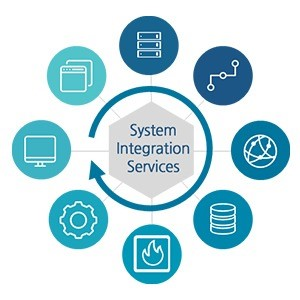
\includegraphics[width=4.5cm]{figures/integrasi.jpg}
		\centering
		\caption{integrasi sistem}
	\end{figure}
	
Sistem integrasi memanfaatkan berbagai Teknik dalam mengintegrasikan dua sistem seperti jaringan computer, integrase aplikasi enterprise, manajemen proses bisnis atau pengguna pemrograman. 
Didunia modern yang terhubung oleh internet integrase sistem sangat memiliki peran penting. Semakin banyak sistem dirancang untuk terhubung, baik dalam sistem yang akan dibangun maupun ke sistem yang sudah digunakan.

Integrasi Sistem Informasi sering disebut Enterprise Information System, yaitu sebuah platform teknologi yang memungkinkan organisasi mengintegrasikan dan mengkoordinasikan proses bisnis. Sedangkan Sandoe (2001) mengatakan bahwa integrasi Sistem Informasi bertujuan menggabungkan Sistem Informasi yang tadinya terpisah dengan tujuan sebuah sumber daya informasi yang lebih komplit dan menyeluruh bagi sebuah organisasi.

\subsection{PHP}
	\begin{figure}[H]
		
\includegraphics[width=4.5cm]{figures/php2.png}
		\centering
		\caption{apa itu php?}
	\end{figure}

PHP merupakan salah satu dari sekian banyak bahasa pemrograman web yang paling umum digunakan dalam pengembangan suatu web. Biasanya dalam implementasinya PHP sering digabungkan atau disisipkan dalam dokumen HTML. PHP memiliki kepanjangan yaitu PHP: Hypertext Preprocessor.Bahasa pemrograman ini bersifat server-side. Arti dari Server-side programming sendiri yaitu script/program tersebut akan dijalankan/diproses oleh server.
\subsubsection{Sejarah PHP}
\hfill\\
Pada awalnya PHP merupakan kependekan dari Personal Home Page (Situs personal). PHP pertama kali dibuat oleh Rasmus Lerdorf pada tahun 1995. Pada waktu itu PHP masih bernama Form Interpreted (FI), yang wujudnya berupa sekumpulan skrip yang digunakan untuk mengolah data formulir dari web.

Selanjutnya Rasmus merilis kode sumber tersebut untuk umum dan menamakannya PHP/FI. Dengan perilisan kode sumber ini menjadi sumber terbuka, maka banyak pemrogram yang tertarik untuk ikut mengembangkan PHP.

Pada November 1997, dirilis PHP/FI 2.0. Pada rilis ini, interpreter PHP sudah diimplementasikan dalam program C. Dalam rilis ini disertakan juga modul-modul ekstensi yang meningkatkan kemampuan PHP/FI secara signifikan.

Pada tahun 1997, sebuah perusahaan bernama Zend menulis ulang interpreter PHP menjadi lebih bersih, lebih baik, dan lebih cepat. Kemudian pada Juni 1998, perusahaan tersebut merilis interpreter baru untuk PHP dan meresmikan rilis tersebut sebagai PHP 3.0 dan singkatan PHP diubah menjadi akronim berulang PHP: Hypertext Preprocessing.

Pada pertengahan tahun 1999, Zend merilis interpreter PHP baru dan rilis tersebut dikenal dengan PHP 4.0. PHP 4.0 adalah versi PHP yang paling banyak dipakai pada awal abad ke-21. Versi ini banyak dipakai disebabkan kemampuannya untuk membangun aplikasi web kompleks tetapi tetap memiliki kecepatan dan stabilitas yang tinggi.

Pada Juni 2004, Zend merilis PHP 5.0. Dalam versi ini, inti dari interpreter PHP mengalami perubahan besar. Versi ini juga memasukkan model pemrograman berorientasi objek ke dalam PHP untuk menjawab perkembangan bahasa pemrograman ke arah paradigma berorientasi objek. Peladen web bawaan ditambahkan pada versi 5.4 untuk mempermudah pengembang menjalankan kode PHP tanpa menginstal peladen perangkat lunak.

Versi terbaru dan stabil dari bahasa pemograman PHP saat ini adalah versi 7.4.3 yang dirilis pada tanggal 20 Februari 2020.

\subsubsection{Sekilas tentang pembuat PHP: Rasmus Lerdorf}
\hfill\\
	\begin{figure}[H]
		
\includegraphics[width=6cm]{figures/web/rasmus.jpg}
		\centering
		\caption{Creator PHP Rasmus Lerdorf }
	\end{figure}
	
Rasmus Lerdorf merupakan seorang programmer yang berasal dari Denmark. Dia membuat dan membantu dalam hal pengkodean bahasa PHP, terutama pada 2 versi awal yang kemudian dikembangkan secara grup bersama dengan Jim Winstead (Yang membuat blo.gs), Stig Bakken, Shane Caraveo, Andi Gutmans, dan juga Zeev Suraski. sampai sekarang ia terus berkontribusi pada projek.

Lerdorf lahir di pulau disko di daerah Greenland dan kemudian pindah ke Denmark pada awal hidupnya. kelaurganya pindah dari Kanada ke Denmark pada tahun 1980, lalu pindah lagi ke kota King di Ontario pada tahun 1983. Dia lulus dari SMA King City pada tahun 1988, dan pada tahun 1993 lulus dari Universitas Waterloo dengan gelar  Bachelor of Applied Science di bidang teknik desain sistem. Dia juga ikut berkontribusi dalam Apache HTTP Server dan menambahkan clausa Limit pada mSQL DBMS. 

Dari Septermber 2002 sampai November 2009, Lerdorf bekerja di perusahaan Yahoo sebagai Infrastructure Architecture Engineer. Pada tahun 2010 kemudian bergabung ke perusahaan WePay untuk mengembangkan API (Application Programming Interface). dan pada tahun 2011 ia menjadi seorang konsultan untuk beberapa startup. Kemudian pada 22 Februari 2012 ia bergabung dengan Etsy, sebuah website e-commerce yang berfokus pada hal hal vintage. Dan pada tahun 2013, Rasmus bergabung dengan Jelastic sebagai Senior Advisor untuk membantu mereka mengembangkan teknologi baru.

Selain itu Lerdorf juga sering menjadi pembicara dalam konferensi open source di berbagai belahan dunia. Beberapa topik yang sering dia bahas diantaranya adalah security vulnerabilities dan juga tentang PHP.

Pada tahun 2003, ia di beri penghargaan oleh MIT Technology Review sebagai salah satu dari 100 inovator di dunia yang berada dibawah umur 35

\subsubsection{Website yang menggunakan PHP} 
\hfill\\
	\begin{figure}[H]
		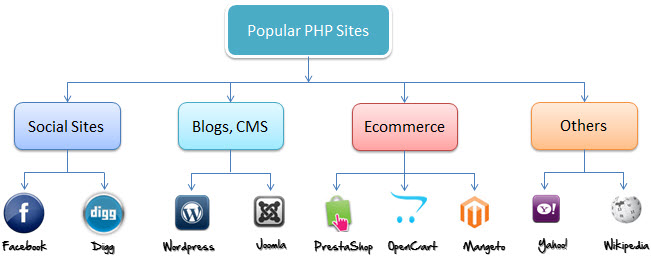
\includegraphics[width=8cm]{figures/web/popularphpsites.jpg}
		\centering
		\caption{Website dengan bahasa PHP}
	\end{figure}

\subsubsection{Contoh Kode PHP}
\hfill\\
	\begin{figure}[H]
		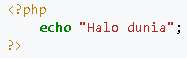
\includegraphics[width=6cm]{figures/web/contohkodingphp.png}
		\centering
		\caption{Program Hello world yang ditulis dengan PHP}
	\end{figure}
\subsubsection{Kelebihan PHP}
\hfill\\
\begin{enumerate}
	\item Bahasa Pemrograman PHP dapat ditemukan di mana - mana.
	\item Proses pengembangan lebih mudah, karena komunitas yang bisa dibilang besar dan mendukung.
	\item PHP adalah bahasa scripting yang paling mudah karena memiliki referensi yang banyak dan lengkap.
	\item PHP adalah bahasa open source yang dapat digunakan di berbagai mesin (Linux, Unix, Macintosh, Windows).
	\item Ringkas dan ringan
	\item Maintenanace Mudah
\end{enumerate}

\subsubsection{Kekurangan PHP}
\hfill\\
\begin{enumerate}
	\item Banyak kompetisi, karena PHP adalah bahasa pemrograman yang paling umum
	\item Terkesan kurang prestigious.
	\item Tidak ideal jika untuk pengembangan skala besar.
	\item PHP mempunyai kelemahan security tertentu.
\end{enumerate}

\subsubsection{Referensi belajar PHP}
\hfill\\
\begin{enumerate}
	\item php.net
	\item sitepoint.com
	\item tutorialspoint.com/php/
\end{enumerate}
	
\subsection{HTML}
	\begin{figure}[H]
		
\includegraphics[width=10cm]{figures/html.jpg}
		\centering
		\caption{Ilustrasi HTML}
	\end{figure}
HTTP merupakan protokol yang digunakan untuk mentransfer data antara web server ke web browser. Protokol ini mentransfer dokumen-dokumen web yang ditulis atau berformat HTML. Dikatakan markup karena HTML berfungsi untuk '' mepercantik " file text biasa untuk ditampilkan pada program web browser. Hal ini dilakukan dengan menambahakan tag-tag (perintah khusus) pada file teks biasa tersebut.

Tag HTML biasanya berupa tag-tag yang berpasang pasangan dan ditandai dengan simbol <dan>. Pasangan dari sebuah sebuah tag ditandai dengan tanda '/ '. misalnya awalnya perintah tagnya <contoh> maka diakhiri dengan </contoh>.

	Supaya dapat menghasilkan tampilan wujud yang terintegerasi Pemformatan hiperteks sederhana ditulis dalam berkas format ASCII sehingga menjadi halaman web dengan perintah-perintah HTML.
HTML merupakan sebuah bahasa yang bermula bahasa yang sebelumnya banyak dipakai di dunia percetakan dan penerbirtan yang disebut Standard Generalized Markup Language (SGML).
	
	Sekarang ini HTML merupakan standar Internet yang dikendalikan dan didefinisikan pemakaiannya oleh World Wide Web Consortium (W3C). Pada tahun 1989, HTML dibuat oleh kolaborasi Berners-lee Robert dengan Caillau TIM pada saat mereka bekerja di CERN (CERN merupakan lembaga penelitian fisika energi tinggi di Jenewa).

\subsubsection{Sejarah HTML}
\hfill\\
HTML dibuat oleh Tim Berners-Lee, seorang ahli fisika di lembaga penelitian CERN yang berlokasi di Swiss. Dia memiliki ide tentang sistem hypertext yang berbasis internet.

Hypertext merujuk pada teks yang memuat referensi (link) ke teks lain yang bisa diakses langsung oleh viewer. Tim merilis versi pertama HTML pada tahun 1991, dan di dalamnya terdiri atas 18 HTML tag. Sejak saat itu, setiap kali bahasa HTML merilis versi teranyarnya, selalu ada tag dan attribute (tag modifier) terbaru.

Berdasarkan HTML Element Reference milik Mozilla Developer Network, untuk saat ini, ada 140 HTL tag meskipun sebagiannya sudah usang (tidak lagi didukung oleh versi terbaru browser).
Berkat popularitasnya yang terus meningkat, HTML kini dianggap sebagai web standard yang resmi. Spesifikasi HTML di-maintain dan dikembangkan oleh World Wide Web Consortiumm (W3C). Cek versi terbaru dari bahasa ini di website W3C.

Upgrade HTML besar-besaran terjadi pada tahun 2014, dan hasilnya adalah pengenalan HTML5. Pada upgrade tersebut, terdapat semantic baru yang memberitahukan arti dari kontennya sendiri, seperti <artcile>, <header>, dan <footer>.


\subsubsection{Fungsi HTML}
\hfill\\
HTML (HyperText Markup Language) adalah suatu bahasa yang menggunakan tanda-tanda tertentu (tag) untuk menyatakan kode-kode yang harus ditafsirkan oleh browser agar halaman tersebut dapat ditampilkan secara benar.
Secara umum, fungsi HTML adalah untuk mengelola serangkaian data dan informasi sehingga suatu dokumen dapat diakses dan ditampilkan di Internet melalui layanan web.
Fungsi HTML yang lebih spesifik yaitu :
\begin{itemize}
\item Membuat halaman web.
\item Menampilkan berbagai informasi di dalam sebuah browser Internet.
\item Membuat link menuju halaman web lain dengan kode tertentu (hypertext).
\item HTTP atau Hypertext Transfer Protokol merupakan protokol yang digunakan untuk mentransfer data atau document yang berformat HTML dari web server ke web browser. Dengan HTTP inilah yang memungkinkan Anda menjelajah internet dan melihat halaman web.
\end{itemize}

\subsubsection{Cara Kerja HTML}
Dokumen HTML adalah file yang diakhiri dengan ekstensi .html atau .htm. Ekstensi file ini bisa dilihat dengan mengunakan web browser apa pun (seperti Google Chrome, Safari, atau Mozila Firefox). Browser tersebut membaca file HTML dan me-render kontennya sehingga user internet bisa melihat dan membacanya.
Biasanya, rata-rata situs web menyertakan sejumlah halaman HTML yang berbeda-beda. Contohnya, beranda utama, halaman ‘tentang kami’, halaman kontak yang semuanya memiliki dokumen HTML terpisah.
Masing-masing halaman HTML terdiri atas seperangkat tags (bisa disebut juga elements), yang mengacu pada building block halaman website. Tag tersebut membuat hirarki yang menyusun konten hingga menjadi bagian, paragraf, heading, dan block konten lainnya.
Sebagian besar element HTML memiliki tag pembuka dan penutup yang menggunakan syntax <tag></tag>.
Berikut contoh kode dari susunan atau struktur HTML:
\lstinputlisting[firstline=1, lastline=8]{src/coba.html}	

Elemen teratas dan terbawah adalah division sederhana (<div></div>) yang bisa Anda gunakan untuk mark up bagian konten yang lebih besar.
Susunan HTML di atas terdiri atas heading (<h1></h1>), subheading (<h2></h2), dua paragraf (<p></p>), dan satu gambar (<img>).
Paragraf kedua meliputi sebuah link (<a></a>) dengan attribute href yang terdiri atas URL tujuan.
Tag gambar memiliki dua attribute, src untuk path gambar dan alt untuk deskripsi gambar.

	
	
	
	
	
\subsection{Framework}
	\begin{figure}[H]
		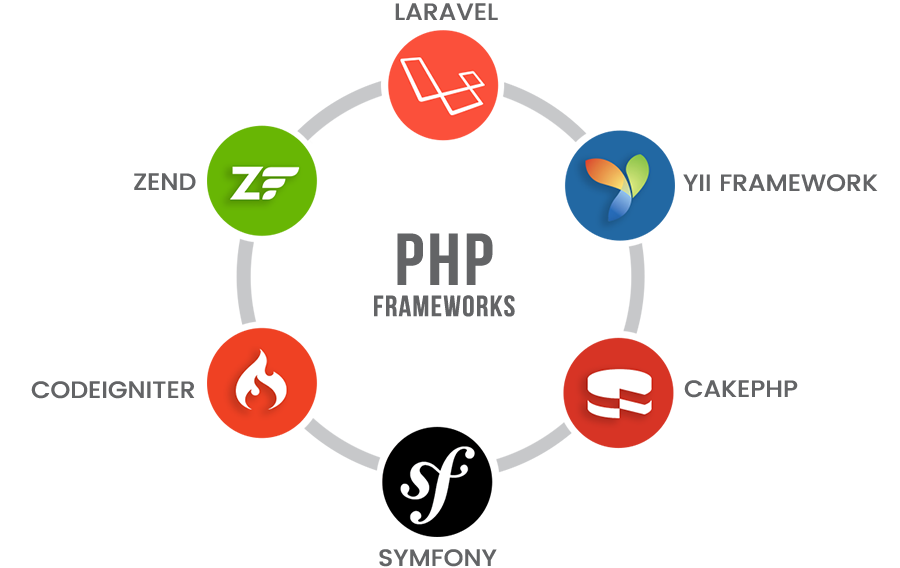
\includegraphics[width=10cm]{figures/web/phpframework.png}
		\centering
		\caption{Framework PHP}
	\end{figure}
PHP Framework adalah suatu kerangka keja yang telah terbentuk dan tersusun untuk memudahkan proses pengembangan website  secara profesional.

Namun perlu diketahui, bahwa PHP Framework memiliki perbedaannya tersendiri jika dibandingkan dengan sebuah CMS (Content Management System). Meskipun pada dasarnya mereka sama-sama memudahkan dalam hal yang sama yaitu pembuatan website. Tetapi untuk CMS  kita tidak perlu repot-repot dan pusing-pusing menulis script maupun sekumpulan kode. Dengan fitur CMS, semuanya telah dibuat instan dan kita hanya perlu sedikit mengatur bagian konten dan interface-nya saja.

Berbeda dengan Framework, kita tetap harus menuliskan script dan sekumpulan kode untuk dapat membangun sebuah web. 

\subsubsection{Mengapa harus menggunakan Framework?}
\hfill\\
\begin{itemize}
	\item Mempercepat proses pengembangan web
	\item Kode yang terorganisir dan dapat digunakan terus menerus (reusable).
	\item Lebih mudah dalam proses maintenance.
	\item Lebih aman dalam hal sekuriti
	\item Menggunakan pola MVC (model - view - controller) yang memisahkan antara presentation dan logic
	\item Konsep web development modern seperti object oriented programming.

\end{itemize}


\subsection{MYSQL(\textit{My Structure Query Language})}
MySQL adalah sebuah server database open source yang terkenal yang digunakan berbagai aplikasi terutama untuk server atau membuat web. MySQL juga adalah sebuah implementasi dari sistem manajemen basis data relasional (RDBMS). Kehandalan suatu sistem basis data (DBMS) dapat diketahui dari cara kerja pengoptimasinya dalam melakukan proses perintah-perintah SQL yang dibuat oleh pengguna maupun program-program aplikasi yang memanfaatkannnya.

Berdasarkan dari pengertian diatas kesimpulan dari MySQL adalah sekumpulan sistem database yang banyak digunakan untuk pengembangan suatu aplikasi berbasis web dan bersifat open source.
MySQL merupakan software yang tergolong sebagai DBMS (Database Management System) yang bersifat Open Source. Open Source menyatakan bahwa software ini dilengkapi dengan source code. MySQL pada awalnya dibuat oleh perusahaan konsultan bernama TcX yang berlokasi di Swedia. Saat ini pengembangan MySQL berada dibawah naungan perusahaan MySQL AB (Kadir, 2008:2).

Fitur yang terdapat pada MySQL:
\begin{enumerate}
	\item \textit{Multipatform}

MySQL tersedia pada beberapa platform (Windows, Linux, Unix dan lain-lain).

	\item Andal
	
cepat dan mudah digunakan MySQL tergolong sebagai database server yang andal, dapat menangani database yang besar dengan kecepatan tinggi, mendukung banyak sekali fungsi untuk mengakses database, dan sekaligus mudah untuk digunakan.

	\item Jaminan keamanan akses
	
MySQL mendukung pengamanan database dengan berbagai kriteria pengaksesan.

	\item Dukungan SQL
	
MySQL mendukung perintah SQL (\textit{Structurd Query Language}). Sebagai diketahui, SQL merupakan standar dalam pengaksesan database relasional.
\end{enumerate}

\subsubsection{Perkembangan MySQL}
\hfill\\
Pada bulan Mei 1996, MySQL versi 1.0 berhasil dirilis secara terbatas hanya utnuk 4 orang sja. Namun di bulan Oktober pada tahun yang sama versi 3.11.0 dilepas ke publik. Namun mula-mula kode ini tidak diberikan dibawah lisensi GPL (General Public License), melainkan lisensi khusus. Pada tahun 1998-1999, yaitu pada versi-versi akhir 3.22, MySQL menjadi semakin populer dan dilirik orang karena kestabilan dan kecepatan yang meningkat. Jika pada versi 3.22, MySQL mulai diadopsi oleh banyak orang. Berbeda halnya dengan versi 3.23 dan 4.0 yang telah terjadi banyak peningkatan dari sisi teknologi (Sukarno, 2006:5-7).

MySQL memiliki beberapa keistimewaan, antara lain : 
\begin{itemize}
\item Portabilitas, MySQL dapat berjalan stabil pada berbagai sistem operasi seperti Windows, Linux, FreeBSD, Mac Os X Server, Solaris, Amiga, dan masih banyak lagi. 
\item Perangkat lunak sumber terbuka. MySQL didistribusikan sebagai perangkat lunak sumber terbuka, dibawah lisensi GPL sehingga dapat digunakan secara gratis.
\item Multi-user. MySQL dapat digunakan oleh beberapa pengguna dalam waktu yang bersamaan tanpa mengalami masalah atau konflik.
\item Performance tuning, MySQL memiliki kecepatan yang menakjubkan dalam menangani query sederhana, dengan kata lain dapat memproses lebih banyak SQL per satuan waktu. 
\item Ragam tipe data. MySQL memiliki ragam tipe data yang sangat kaya, seperti signed / unsigned integer, float, double, char, text, date, timestamp, dan lainlain.
\item Perintah dan Fungsi. MySQL memiliki operator dan fungsi secara penuh yang mendukung perintah Select dan Where dalam perintah (query).
\item Keamanan. MySQL memiliki beberapa lapisan keamanan seperti level subnetmask, nama host, dan izin akses user dengan sistem perizinan yang mendetail serta sandi terenkripsi. 
\item Skalabilitas dan Pembatasan. MySQL mampu menangani basis data dalam skala besar, dengan jumlah rekaman (records) lebih dari 50 juta dan 60 ribu tabel serta 5 milyar baris. Selain itu batas indeks yang dapat ditampung mencapai 32 indeks pada tiap tabelnya.
\item Konektivitas. MySQL dapat melakukan koneksi dengan klien menggunakan protokol TCP/IP, Unix soket (UNIX), atau Named Pipes (NT).
\item Lokalisasi. MySQL dapat mendeteksi pesan kesalahan pada klien dengan menggunakan lebih dari dua puluh bahasa. Meski pun demikian, bahasa Indonesia belum termasuk di dalamnya. 
\item Antar Muka. MySQL memiliki antar muka (interface) terhadap berbagai aplikasi dan bahasa pemrograman dengan menggunakan fungsi API (Application Programming Interface).
\item Klien dan Peralatan. MySQL dilengkapi dengan berbagai peralatan yang dapat digunakan untuk administrasi basis data, dan pada setiap peralatan yang ada disertakan petunjuk online.\
\item Struktur tabel. MySQL memiliki struktur tabel yang lebih fleksibel dalam menangani ALTER TABLE, dibandingkan basis data lainnya semacam PostgreSQL ataupun Oracle

\end{itemize}

\subsection{Pengenalan Codeigniter}
	\begin{figure}[H]
		
\includegraphics[width=4.5cm]{figures/codeigniter.png}
		\centering
		\caption{Logo Codeigniter}
	\end{figure}
CodeIgniter sendiri merupakan salah satu framework php yang bersifat aplikasi sumber terbuka(Open Source) dengan model MVC (Model, View, Controller) yang digunakan untuk mengembangkan situs web yang dinamis. CodeIgniter mempermudah proses pengembang web untuk membuat aplikasi web dengan waktu yang lebih cepat dan mudah dibandingkan dengan membuatnya dari awal. CodeIgniter dirilis pertama kali pada 28 Februari 2006. 

\subsubsection{Konsep MVC (Model View dan Controller)}
\hfill\\
	\begin{figure}[H]
		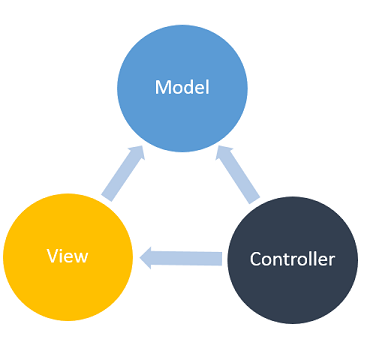
\includegraphics[width=8cm]{figures/web/mvc.png}
		\centering
		\caption{MVC Concept}
	\end{figure}
Model View Controller merupakan suatu konsep yang cukup populer dalam mengembangkan suatu aplikasi web, Konsep MVC ini mencoba memisahkan pengembangan aplikasi berdasarkan komponen-komponen utama dalam membuat suatu aplikasi seperti misalkan bagian untuk pemrosesan/manipulasi data, tampilan , dan bagian untuk kontrol aplikasi. Terdapat 3 jenis komponen yang membangun suatu pola MVC dalam suatu aplikasi yaitu: 
\begin{enumerate}
	\item View, merupakan bagian yang akan ditampilkan dan dilihat oleh pengguna. Biasanya, yang ditampilkan adalah dokumen HTML yang diatur oleh controller. View berfungsi untuk menerima dan merepresentasikan data kepada pengguna. Bagian view tidak dapat memiliki akses pada bagian model.
	\item Model, Berhubungan langsung dengan proses CRUD (Create, Read, Update, Delete), serta search. Model juga menangani validasi dari bagian controller, tetapi berhubungan langsung dengan view.
	\item Controller, merupakan bagian yang menghubungkan model dan juga view, controller berperan dalam menerima data dari view kemudian memprosesnya untuk dikirim ke bagian model.
\end{enumerate}

\subsubsection{Kelebihan dan Kekurangan Codeigniter}
\hfill\\
\begin{enumerate}
\item Kelebihan
	\begin{itemize}
	\item Performa sangat cepat.
	\item Konfigurasi yang sangat minim
	\item Komunitas yang aktif dan mendukung
	\item Dokumentasi yang sangat lengkap
	\end{itemize}
\item Kekurangan
\begin{itemize}
	\item CodeIgniter tidak ditujukan untuk pembuatan web dengan skala besar.
	\item Tidak Adanya Editor Khusus.
\end{itemize}
\end{enumerate}

\subsubsection{Instalasi Codeigniter}
\hfill\\
\begin{itemize}
	\begin{figure}[H]
		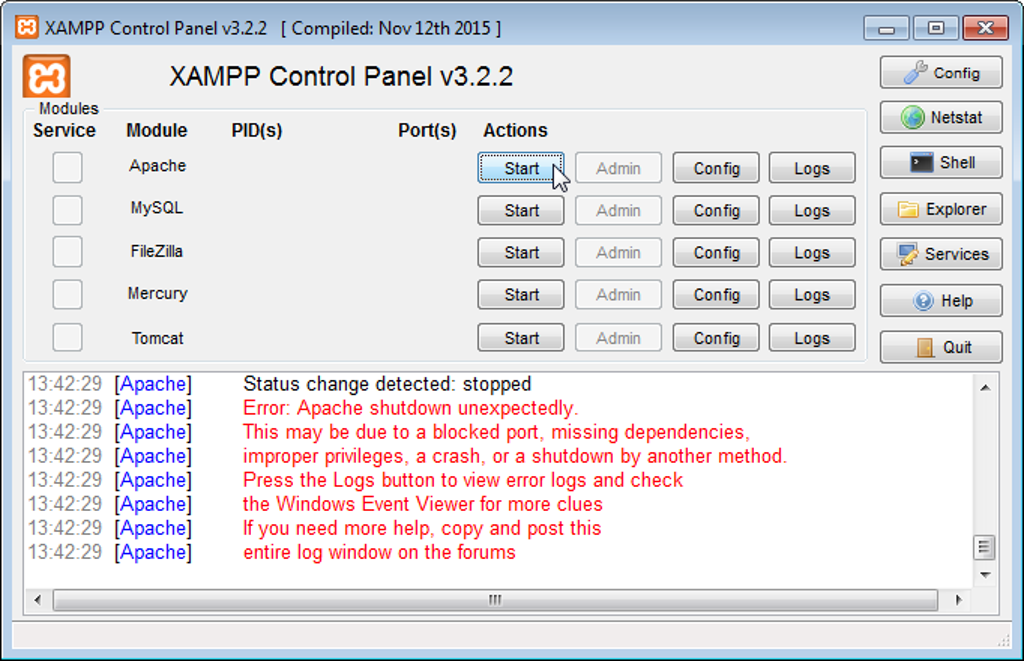
\includegraphics[width=8cm]{figures/web/Xampp.png}
		\centering
		\caption{Tampilan Xampp}
	\end{figure}
	\item Download Xampp terlebih dahulu di https://www.apachefriends.org/
	\item Kemudian install Xampp(untuk lebih jelas silahkan buka bab Instalasi dan penggunaan tools yang digunakan)
	\begin{figure}[H]
		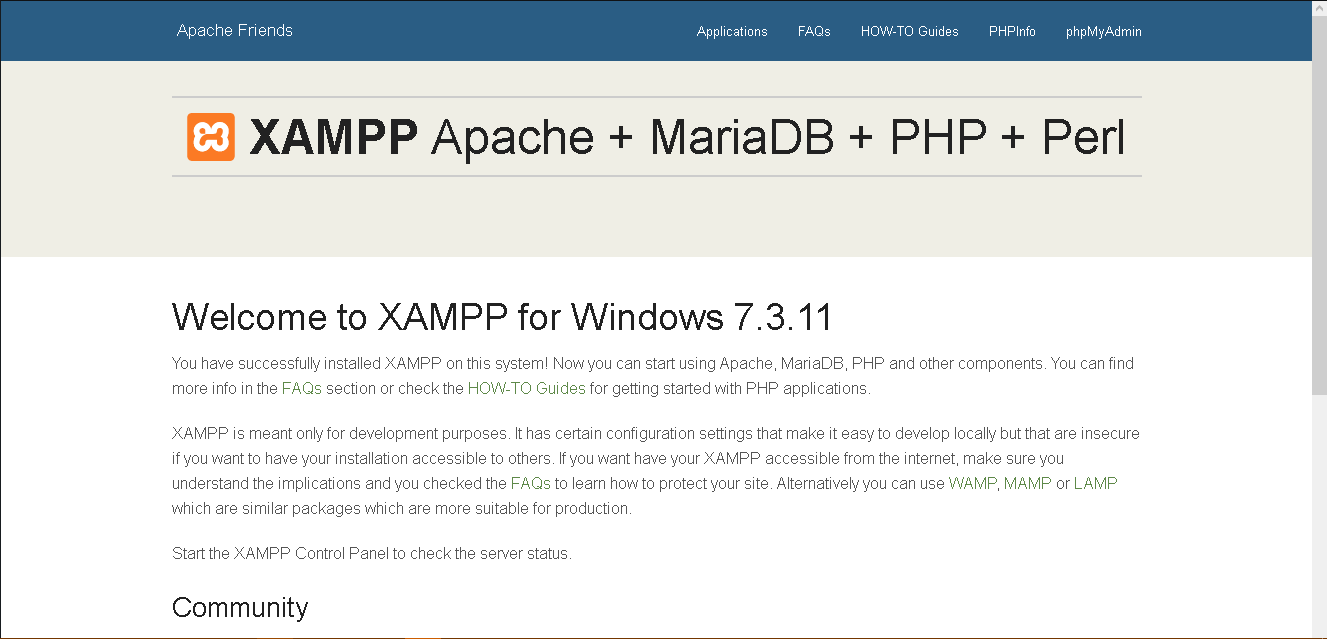
\includegraphics[width=8cm]{figures/web/tampilanwebxampp.png}
		\centering
		\caption{Tampilan web Xampp jika berhasil instalasi}
	\end{figure}


	\begin{figure}[H]
		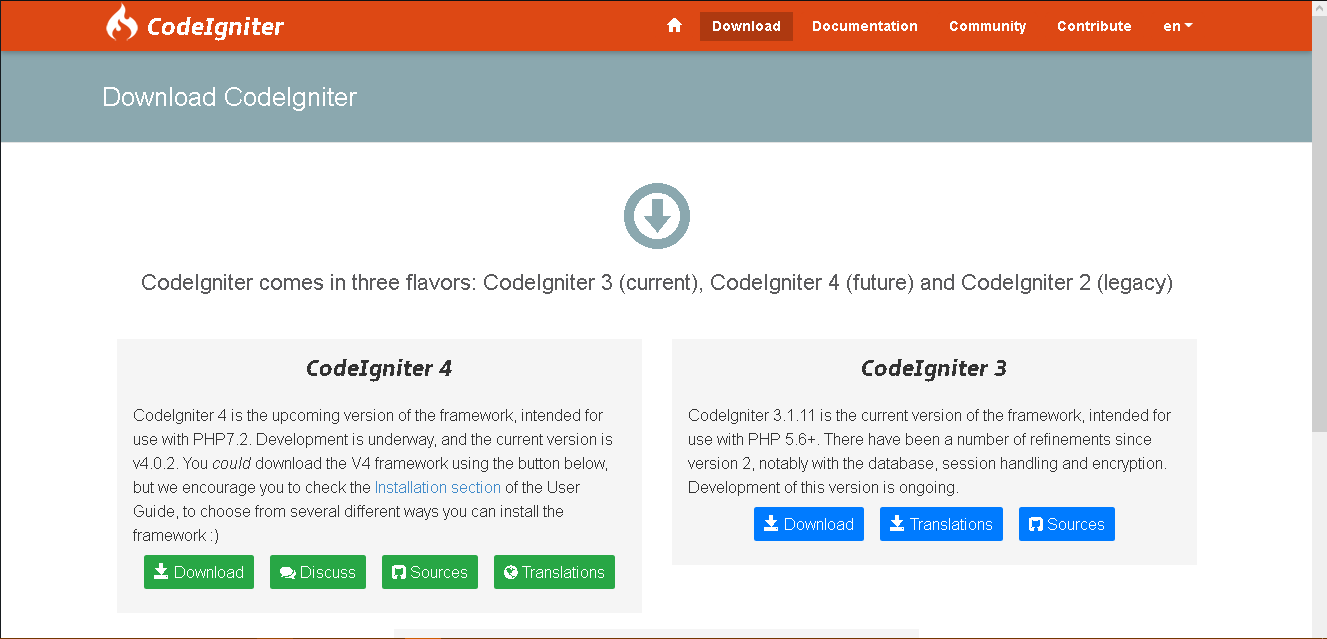
\includegraphics[width=8cm]{figures/web/websitecodeigniter.png}
		\centering
		\caption{Website Codeigniter}
	\end{figure}
	\item Kemudian, dilanjutkan dengan instalasi codeigniter dengan cara mendownload terlebih dahulu codeigniter-nya di https://codeigniter.com/en/download


	\begin{figure}[H]
		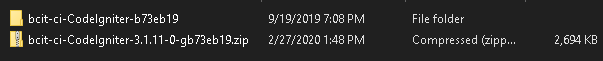
\includegraphics[width=8cm]{figures/web/ekstrakcodeigniter.png}
		\centering
		\caption{Ekstrak File}
	\end{figure}
	\item ekstrak file yang telah di download

	\item berikut adalah hasil ekstrak file
	\begin{figure}[H]
		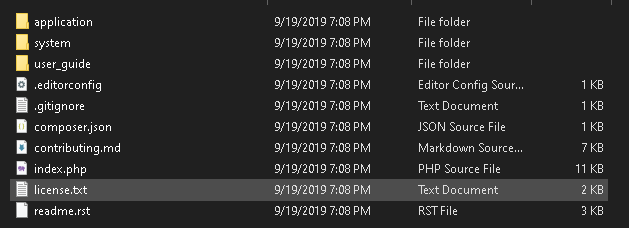
\includegraphics[width=8cm]{figures/web/hasilekstrakcodeigniter.png}
		\centering
		\caption{Hasil Ekstrak File}
	\end{figure}

	\item Setelah itu pindahkan folder yang telah di extract tadi kedalam folder htdocs (C:/xampp/htdocs)
	\begin{figure}[H]
		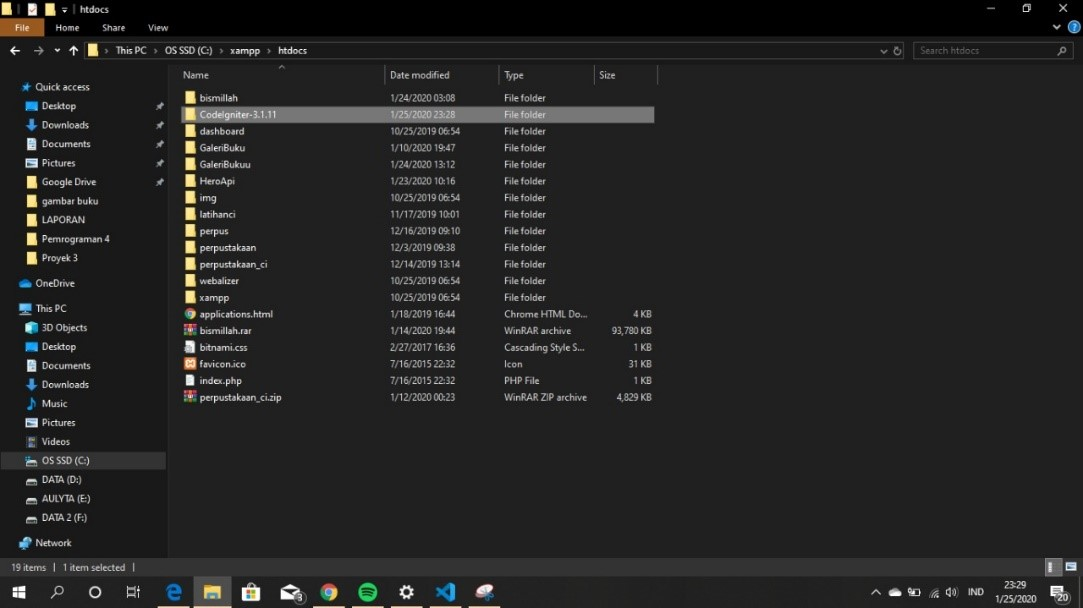
\includegraphics[width=8cm]{figures/instalasi/ci1.jpg}
		\centering
		\caption{Membuka Direktory htdocs}
	\end{figure}	

	\item Kemudian ubah nama file tersebut sesuai dengan yang anda inginkan, disini saya menggunakan nama file contohCI.	
		
	\item Setelah itu buka aplikasi Xampp dan jalankan xampp dengan  mengklik pada bagian actions sampai berubah menjadu stop.
	\begin{figure}[H]
		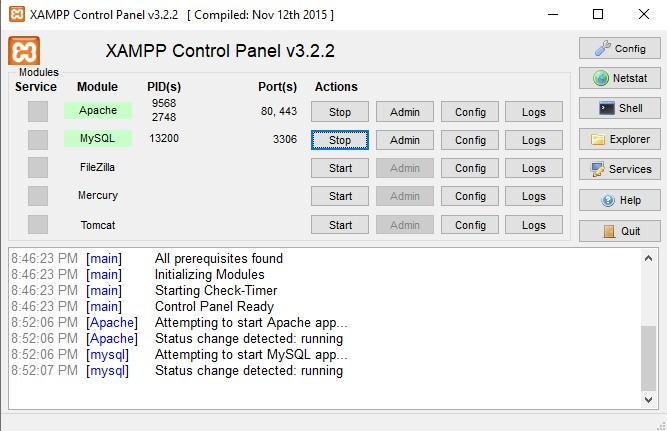
\includegraphics[width=8cm]{figures/instalasi/ci2.jpg}
		\centering
		\caption{Menjalankan XAMPP}
	\end{figure}	
	
	\item Selanjutnya buka browser dan ketikkan  http://localhost/contohci/
	\begin{figure}[H]
		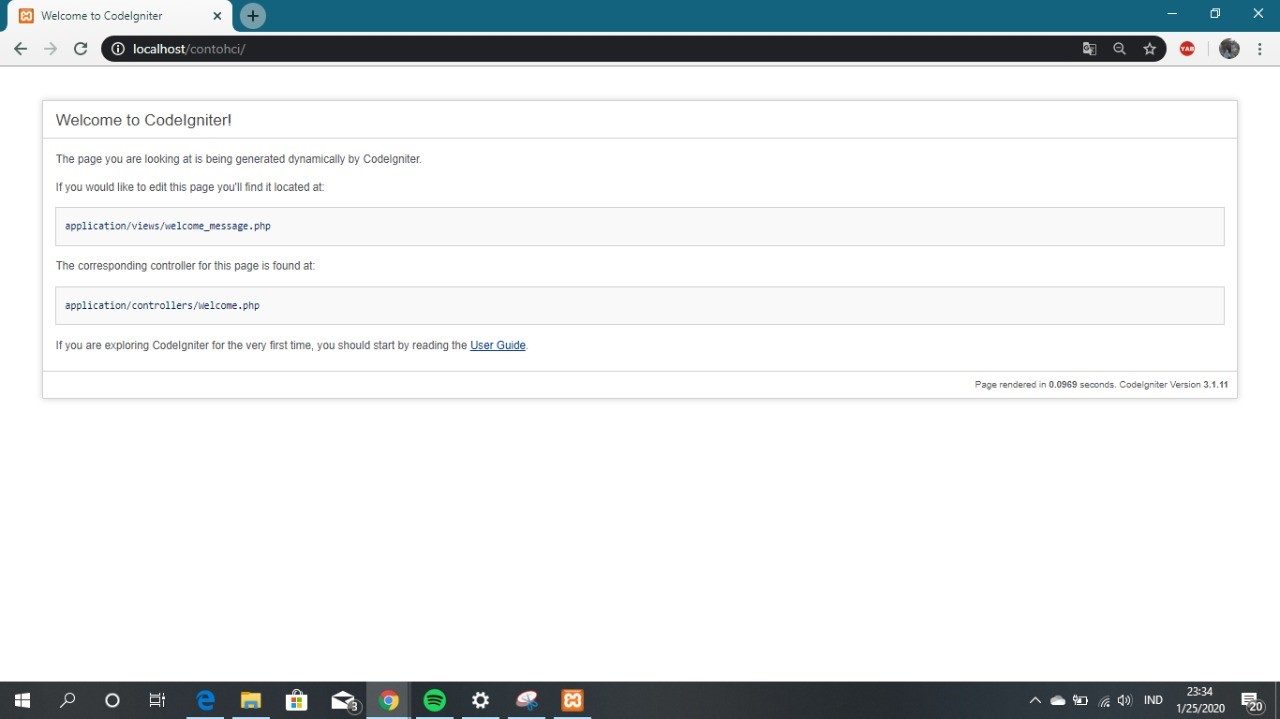
\includegraphics[width=8cm]{figures/instalasi/ci3.jpg}
		\centering
		\caption{Mencobanya di browser}
	\end{figure}	
	
	\item Selamat codeigniter berhasil di install.
	\item Setelah itu buka VisualCode yang telah di install tadi, hal ini dilakukan untuk mengenali struktur direktori pada codeigniter.
Berikut adalah struktur direktori codeigniter
	\begin{figure}[H]
		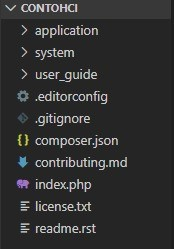
\includegraphics[width=8cm]{figures/instalasi/ci4.jpg}
		\centering
		\caption{Struktur direcory dari Codeigniter}
	\end{figure}
	Terdapat dua direktori penting didalam CI yaitu folder application dan folder System . selain juga terdapat direktori folder user\_ guide dan beberaopa file. Berikut adalah beberapa penjelasan yang terdapat dalam CI:	
	\begin{itemize}
		\item Folder Application
		\hfill\\
		\begin{figure}[H]
			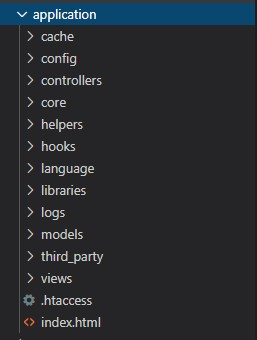
\includegraphics[width=8cm]{figures/instalasi/ci5.jpg}
			\centering
		\caption{Struktur direcory dari folder Application}
	\end{figure}
		Folder application berisi code aplikasi. Disinilah kita akan menulis semua baris kode aplikasi yang akan kita bangun. Dalam folder application terdapat beberapa direktori yaitu:
		\begin{itemize}
			\item Folder chace, adalah suatu folder yang berisi chace dari aplikasi.
			\begin{figure}[H]
				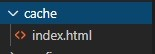
\includegraphics[width=8cm]{figures/instalasi/ci6.jpg}
				\centering
				\caption{Folder Application/cache}
			\end{figure}
			
			\item Folder config, adalah suatu folder yang berisi konfigurasi aplikasi. 
			\begin{figure}[H]
				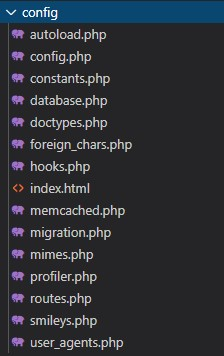
\includegraphics[width=8cm]{figures/instalasi/ci7.jpg}
				\centering
				\caption{Folder Application/config}
			\end{figure}	
			\begin{enumerate}
				\item Auotoload.php, merupakan suatu tempat yang mendefinisikan autoload.
				\item Config.php, adalah suatu file untuk mengkonfigurasi aplikasi.
				\item Constants.php, merupakan suatu file yang berisi konstanta.
				\item Database.php, merupakan suatu file yang berisi konfiguarsi database aplikasi.
				\item Doctypes.php, adalah suatu file yang berisi definisi untuk doctype html.
				\item Foreign\_ chars.php, merupakan suatu file yang berisi character dan symbol.
				\item Hooks.php, merupakan suatu file yang berisi konfigurasi hooks.
				\item Index.html, merupakan suatu file untuk mencegah direct access.
				\item Memchaced.php , merupakan suatu file yang berisi suatu konfigurasi untuk menchace.
				\item Migration.php, merupakan suatu file yang berisi untuk migrasi.
				\item Mimes.php, merupakan suatu file yang berisi definisi type file
				\item Profiler.php, merupakan suatu file yang berisi konfigurasi untuk profiler.
				\item Routes.php, merupakan suatu file yang digunakan sebagai tempat untuk menulis route aplikasi.
				\item Smileys.php, berisi kode untuk emoji.
				\item User\_ agents.php, merupakan suatu file yang berisi definisi untuk user\_ agents.
			\end{enumerate}
			
			\item Folder Controllers, merupakan suatu folder yang berisi kode-kode controller.
			\begin{figure}[H]
				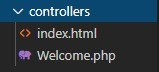
\includegraphics[width=8cm]{figures/instalasi/ci17.jpg}
				\centering
				\caption{Folder Application/controllers}
			\end{figure}			

			\item Folder Core, merupakan suatu folder yang berisi kode-koed untuk coustome core..
			\begin{figure}[H]
				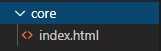
\includegraphics[width=8cm]{figures/instalasi/ci18.jpg}
				\centering
				\caption{Folder Application/core}
			\end{figure}
		
			\item Folder Helpers, merupakan suatu folder adalah fungsi-fungsi helper.
			\begin{figure}[H]
				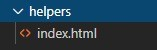
\includegraphics[width=8cm]{figures/instalasi/ci19.jpg}
				\centering
				\caption{Folder Application/helpers}
			\end{figure}
			
			\item Folder Hooks, meruapakan suatu folder yang berisi kode untuk script hook.
			\begin{figure}[H]
				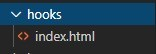
\includegraphics[width=8cm]{figures/instalasi/ci20.jpg}
				\centering
				\caption{Folder Application/hooks}
			\end{figure}
			
			\item Folder language, merupakan suatu folder yang berisi string untuk bahasa apabila web mendukung multi bahasa.
			\begin{figure}[H]
				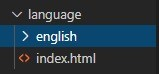
\includegraphics[width=8cm]{figures/instalasi/ci21.jpg}
				\centering
				\caption{Folder Application/config}
			\end{figure}

			\item Folder Libraries, merupakan suatu folder yang berisi library
			\begin{figure}[H]
				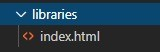
\includegraphics[width=8cm]{figures/instalasi/ci22.jpg}
				\centering
				\caption{Folder Application/libraries}
			\end{figure}			
	
			\item Folder Logs, merupakan suatu folder yang berisi logs dari aplikasi.
			\begin{figure}[H]
				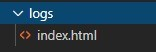
\includegraphics[width=8cm]{figures/instalasi/ci23.jpg}
				\centering
				\caption{Folder Application/logs}
			\end{figure}	

			\item Folder models, berisi kode-kode untuk model
			\begin{figure}[H]
				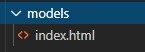
\includegraphics[width=8cm]{figures/instalasi/ci24.jpg}
				\centering
				\caption{Folder Application/model}
			\end{figure}	
	
			\item Folder Third\_ party, merupakan suatu folder yang berisi library dari pihak ketiga
			\begin{figure}[H]
				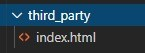
\includegraphics[width=8cm]{figures/instalasi/ci25.jpg}
				\centering
				\caption{Folder Application/third\_ party}
			\end{figure}	
	
			\item Folder Views, merupakan suatu folder yang berisi kode suatu view.
			\begin{figure}[H]
				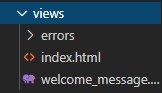
\includegraphics[width=8cm]{figures/instalasi/ci26.jpg}
				\centering
				\caption{Folder Application/views}
			\end{figure}	
		\end{itemize}
		
		\item Folder System, Folder ini berisi kode-kode inti dari codeigniter. Perlu diingat bahwa janganlah anda mengubah apapun didalam direktori ini.jika anda ingin menuprage versi ke yang baru anda cukup mereplace direktori tersebut dengan yang baru.
		\begin{figure}[H]
			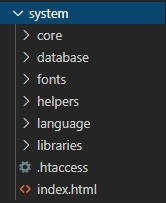
\includegraphics[width=8cm]{figures/instalasi/ci8-1.jpg}
			\centering
			\caption{Folder System/}
		\end{figure}			
		
		\item Folder User\_ guide, Folder ini berisi dokumentasi lengkap dari codeigniter, dengan folder ini kita bisa mengakses dokumentasi CI secara offline. Anda bisa mengapus direktori ini saat web yang anda buat telah jadi.		
		\begin{figure}[H]
			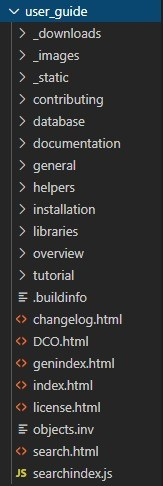
\includegraphics[width=5cm]{figures/instalasi/ci9-1.jpg}
			\centering
			\caption{Folder User\_ guide/}
		\end{figure}	
		
		\item File .editorconfig, File ini berisi konfigurasi untuk text editor.		
		\begin{figure}[H]
			
\includegraphics[width=8cm]{figures/instalasi/ci10.jpg}
			\centering
			\caption{File .editorconfig}
		\end{figure}

		\item File .gitignore, File ini berisi daftar file dan folder yang akan dibaikan oleh git.		
		\begin{figure}[H]
			
\includegraphics[width=8cm]{figures/instalasi/ci11.jpg}
			\centering
			\caption{File .gitignore}
		\end{figure}

		\item File Composer.json, File ini adalah suatu yang berisi keterangan project dan keterangan library yang digunakan, selain itu file ini dibutuhkan oleh composer		
		\begin{figure}[H]
			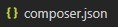
\includegraphics[width=8cm]{figures/instalasi/ci12.jpg}
			\centering
			\caption{File composer.json}
		\end{figure}
		
		\item File Contributing.md, file ini adalah suatu file yang berisi penjelasan tentang cara berkontribusi diproyek CI. File ini dapat dihapus apabila web sudah jadi.		
		\begin{figure}[H]
			
\includegraphics[width=7cm]{figures/instalasi/ci13.jpg}
			\centering
			\caption{File constributing.md}
		\end{figure}		

		\item File Index.php, file ini adalah suatu file utama dari codeigniter yang merupakan file yang akan dibuka pertama kali saat kita mengakses web.		
		\begin{figure}[H]
			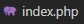
\includegraphics[width=6cm]{figures/instalasi/ci14.jpg}
			\centering
			\caption{File index.php}
		\end{figure}

		\item File license.txt, file ini berisi keterangan lisensi dari codeigniter	
		\begin{figure}[H]
			
\includegraphics[width=6cm]{figures/instalasi/ci15.jpg}
			\centering
			\caption{File license.txt}
		\end{figure}
		
		\item File Readme.rst, File ini sama seperti dengan file contributing.md. file ini berisi penjelasan dan informasi tentangg proyek codeigniter. File ini dapat dihapus saat web sudah selesai.	
		\begin{figure}[H]
			
\includegraphics[width=8cm]{figures/instalasi/ci16.jpg}
			\centering
			\caption{File Readme.rst}
		\end{figure}		
	\end{itemize}
\end{itemize}

\subsubsection{Konfigurasi Dasar Codeigniter}
\hfill\\
Dalam memulai codeigniter ada beberapa konfigurasi yang harus di lakukan pada beberapa file yaitu file autoload.php, file config, dan database.php. Semua konfigurasi tersebut terletak didalam folder appilication/config.
	\begin{figure}[H]
		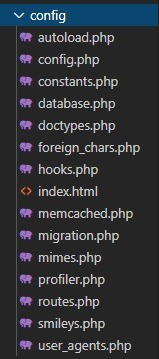
\includegraphics[width=8cm]{figures/instalasi/ci27-1.jpg}
		\centering
		\caption{folder application/config}
	\end{figure}
	\begin{itemize}
	\item Autoload.php
	\hfill\\
	Pada file ini digunakan untuk mengatur fungsi-fngsi yanga akan di muat secara otomatis diawal ketika suatu program dijalankan. Untuk melakukan konfigurasi pada file autoload.php silahkan buka folder application/config/autoload.php.
		\begin{figure}[H]
			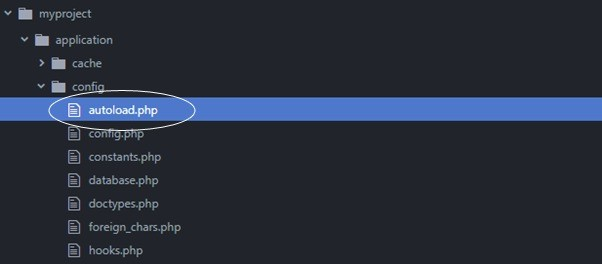
\includegraphics[width=8cm]{figures/instalasi/ci28.jpg}
			\centering
			\caption{autoload.php}
		\end{figure}
		Ada beberapa hal yang bisa di load secara otomatis dalam codeigniter yaitu package, libraries, drivers, helper files, custom config files, language files, dan models.
Untuk konfigurasi dasar yang perlu anda ketahui adalah libraries dan helper files hal tersebut memiliki tujuan agar beberapa library dan helper tertentu berjalan otomatis. 
Untuk melakukan konfigurasi pada libraries buka file autoload.php dengan text editor kemudia temukan kode berikut :
		\begin{figure}[H]
			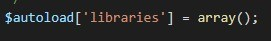
\includegraphics[width=8cm]{figures/instalasi/ci29.jpg}
			\centering
			\caption{autoload.php> libraries}
		\end{figure}
		Setelah itu atur menjadi seperti gambar berikut:
		\begin{figure}[H]
			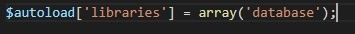
\includegraphics[width=8cm]{figures/instalasi/ci30.jpg}
			\centering
			\caption{autoload.php> libraries hasil}
		\end{figure}
		Pada kode diatas artinya kita akan meload library database secara otomatis, sehingga anda dapat menggunakan fungsi-fungsi database pada codeigniter. 
Selanjutnya kita akan melakukan konfigurasi pada helper files,  kemudian temukan kode berikut:
		\begin{figure}[H]
			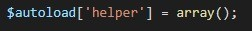
\includegraphics[width=8cm]{figures/instalasi/ci31.jpg}
			\centering
			\caption{autoload.php> helper}
		\end{figure}
		Setelah itu atur menjadi seperti gambar berikut:
		\begin{figure}[H]
			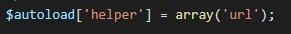
\includegraphics[width=8cm]{figures/instalasi/ci32.jpg}
			\centering
			\caption{autoload.php> helper hasil}
		\end{figure}		
		Pada kode diatas artinya kita akan meload helper URL secara otomatis. Dengan demikian anda dapat menggunakan fungsi-fungsi URL pada codeigniter, misalnya fungsi base\_ url(), site\_ url(), URI Segment, dan sebagainya.
	
	\item Config.php	
	\hfill\\
	Pada file ini terdapat beberapa konfigurasi yang secara standar sudah terkonfiguarasi, namun terdapat beberap konfigurasi yang perlu diperhatikan:
	
	Base\_ url, merupakan url dasar dari project anda. Temukan kode berikut:
		\begin{figure}[H]
			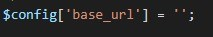
\includegraphics[width=8cm]{figures/instalasi/ci33.jpg}
			\centering
			\caption{autoload.php> base\_ url}
		\end{figure}
		Setelah itu atur menjadi seperti gambar berikut:
		\begin{figure}[H]
			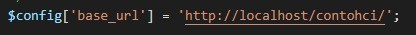
\includegraphics[width=8cm]{figures/instalasi/ci34.jpg}
			\centering
			\caption{autoload.php> base\_ url hasil}
		\end{figure}	
		
	\item Database.php
	\hfill\\
	Dilihat dari nama filenya anda pasti sudah mengetahui apa fungsi dari file ini. File database.php berfungsi untuk melakukan konfigurasi yang berkaitan dengan konfigurasi database dari website  yang akan di buat. Konfigurasi yang perlu diperhatikan tersebut diantaranya: hostname, usename, password, dan database. 
Untuk melakukan konfigurasi pada database.php buka file database.php dengan text editor.
		\begin{figure}[H]
			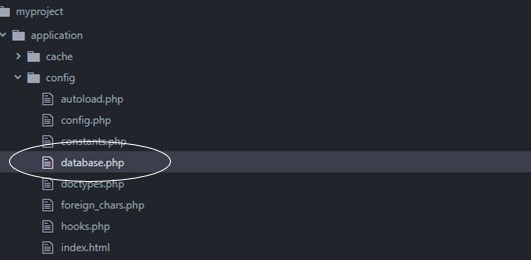
\includegraphics[width=8cm]{figures/instalasi/ci35.jpg}
			\centering
			\caption{database.php}
		\end{figure}
	Kemudian temukan kode berikut :
		\begin{figure}[H]
			\includegraphics[width=8cm]{figures/instalasi/ci36.jpg}
			\centering
			\caption{database.php> default}
		\end{figure}	
		Setelah itu ubah kode tersebut seperti gambar dibawah ini :
		\begin{figure}[H]
			\includegraphics[width=8cm]{figures/instalasi/ci37.jpg}
			\centering
			\caption{database.php> default hasil}
		\end{figure}	
	\end{itemize}

		
\subsection{Pengenalan API}
	\begin{figure}[H]
		\includegraphics[width=8cm]{figures/GambarAPI.png}
		\centering
		\caption{API}
	\end{figure}
API merupakan singkatan yang memiliki kepanjangan yaitu Application Programming Interface, API ini digunakan oleh developer untuk melakukan proses integrasi dua bagian dari satu atau lebeih aplikasi yang berbeda secara bersamaan. API terdiri dari hal-hal seperti function, protocols, dan juga tools. 

Tujuan dari penggunaan API sendiri adalah untuk mempercepat proses pengembangan dari suatu project dengan cara menyediakan beberapa function secara terpisah sehingga para pengembang tidak diperlukan untuk membuat function dengan fungsi tertentu dari awal, langsung pakai saja.

Penerapan API akan memiliki dampak yang signifikan jika fitur yang berkaitan sudah semakin kompleks yang pastinya akan membutuhkan waktu apabila harus memulainya dari awal hanya sekedar untuk membuat function yang memiliki fungsi yang sama dengan API yang telah ada

\subsubsection{Fungsi API}
\hfill\\
API memiliki fungsi untuk menyediakan function yang lebih terstrukur serta terbaca dan mudah dipahami oleh seorang programmer. Hal ini merupakan hal yang krusial, terutama pada bagian editing serta pengembangan suatu projek

\subsubsection{Jenis-Jenis API}
\hfil\\
\begin{itemize}
	\item Ownership Web API
	\item Communication Level API
	\item Web Service API
\end{itemize}

\subsection{UML \textit{Unified Modeling Language}}
\textit{Unified Modeling Language} (UML) adalah standar de facto untuk analisis perangkat lunak berorientasi objek dan pemodelan desain. UML membantu memodelkan berbagai aspek sistem melalui berbagai diagram yang di dukungnya. Setiap aspek dari suatu sistem disajikan dengan menggunakan jenis diagram UML tertentu dan satu set diagrama disebut sebagai model.

UML mempunyai sejumlah elemen grafis yang bisa dikombinasikan menjadi diagram. Karena ini merupakan sebuah bahasa, UML memiliki sejumlah aturan untuk menggabungkan atau mengkombinasikan elemen-elemen tersebut.

\subsubsection{Usecase Diagram}
\hfill\\
Use case diagram menjelaskan apa yang akan dilakukan oleh sistem uang akan dibangun dan siapa yang berinteraksi dengan sistem. Use case diagram menjadi dokumen kesepakatan antara customer, user dan developer. User menggunakan dokumen use case diagram ini untuk memahami sistem dan mengevaluasi bahwa benar yang dilakukan sistem adalah untuk memecahkan masalah yang user ajukan. Use case diagram memberikan gambaran statis dari sistem yang sedang dibangun dan merupakan artifak dari proses analisis (Hermawan, 2004:23).
	\begin{figure}[H]
		\includegraphics[width=8cm]{figures/usecase.jpg}
		\centering
		\caption{Gambar usecase diagram}
	\end{figure}
	
\subsubsection{Class Diagram}
\hfill\\
Class diagram merupakan diagram yang selalu ada di pemodelan sistem berorientasi obyek. Class diagram menunjukkan hubungan antar class dalam sistem yang sedang dibangun dan bagaimana mereka saling berkolaborasi untuk mencapi tujuan. Class diagram digunakan untuk menggambarkan disain statis dari sistem yang sedang dibangun (Hermawan, 2004:27).
	\begin{figure}[H]
		\includegraphics[width=8cm]{figures/classdiagram.jpg}
		\centering
		\caption{Gambar class diagram}
	\end{figure}
	
\subsubsection{Sequence Diagram}
\hfill\\
Sequence diagram menjelaskan secara detail uruta proses yang dilakukan dalam sistem untuk mencapai tujuan dari use case: interaksi yang terjadi antar class, operasi apa saja yang terlibat, urutan antar operasi, dan informasi yang diperlukan oleh masing-masing operasi. Sequence diagram menjelaskan aspek dinamis dari sistem yang sedang dibangun (Hermawan, 2004:24).
	\begin{figure}[H]
		\includegraphics[width=8cm]{figures/sequence.jpg}
		\centering
		\caption{Gambar sequence diagram}
	\end{figure}

\subsubsection{Activity DIagram}
\hfill\\
Activity diagram adalah teknik untuk mendeskripsikan logika prosedural, proses bisnis dan aliran kerja dalam banyak kasus. Activity diagram mempunyai peran seperti halnya flowchart, akan tetapi perbedaannya dengan flowchart adalah activity diagram mendukung perilaku paralel sedangkan flowchart tidak bisa (Munawar, 2005:109).
	\begin{figure}[H]
		\includegraphics[width=8cm]{figures/activity.jpg}
		\centering
		\caption{Gambar activity diagram}
	\end{figure}
	
\subsection{Database}
	\begin{figure}[H]
		\includegraphics[width=8cm]{figures/db.jpg}
		\centering
		\caption{Gambaran Database}
	\end{figure}
Database didefinisikan sebagai kumpulan data yang saling berkaitan secara teknis, database juga sebagai tempat media penyimpanan data kita dalam membuat sebuah program yang berisikan tabel, field, record, yang diselimuti dengan DBMS (Database Management System).
	\begin{figure}[H]
		\includegraphics[width=8cm]{figures/db2.jpg}
		\centering
		\caption{Gambaran Database 2}
	\end{figure}
Basis data (database) ini kumpulan dari data yang saling berhubungan satu dengan lainnya, tersimpan di perangkat keras komputer dan digunakan perangkat lunak untuk memanipulasinya (Jogiyanto, 2005:217). Jadi basis data merupakan suatu komponen utama sistem informasi karena semua informasi untuk pengambilan keputusan berasal dari data di basis data.

Sampai dengan membentuk suatu data base, data mempunyai jenjang yang dapat dilihat pada gambar (Jogiyanto, 1999:714-715): 
\begin{enumerate}
	\item Characters
	\hfill\\
	Characters merupakan bagian data yang terkecil, dapat berupa karakter numerik, huruf atau pun karakter-karakter khusus (special characters) yang membentuk suatu item data atau field.
	
	\item Field
	\hfill\\
	Field menggambarkan suatu atribut dari record yang menunjukkan suatu item dari data, seperti misalnya nama, alamat dan lain sebagainya. Kumpulan dari field membentuk suatu record
	\begin{itemize}
	\item Nama dari field (field name), Field harus diberi nama untuk membedakan field yang satu dengan field yang lain.
	\item Representasi dari field (field representation), Representasi dari field menunjukan tipe dari field (field type) dapat berupa tipe numeric, karakter atau huruf, tanggal, dan memo, serta lebar dari field (field width) menunjukan ruang maksimum dari field yang dapat diisi dengan karakter-karakter data.
	\item Nilai dari field (field value), Nilai dari field menunjukan isi dari field untuk masingmasing record.
	\end{itemize}
	
	\item Records
	\hfill\\
	Record merupakan kumpulan dari field yang membentuk suatu record. Record menggambarkan suatu unit data individu  tertentu. Kumpulan dari record membentuk suatu file. Misalnya file mahasiswa, tiap-tiap record dapat mewakili data tiap-tiap mahasiswa.
	
	\item File
	\hfill\\
	File terdiri dari record-record yang menggambarkan satu kesatuan data yang sejenis. Misalnya file mata kuliah berisi data tentang semua mata kuliah yang ada.
\end{enumerate}

DataBase Management System (DBMS atau DMS) adalah paket perangkat lunak yang komplek digunakan untuk memenipulasi  database (Jogiyanto, 1999:731). Lebih detail lagi dijelaskan oleh Hariyanto bahwa DBMS adalah perangkat lunak untuk mendefinisikan, menciptakan, mengelola dan mengendalikan pengaksesan basisdata. Semua operasi input dan output yang berhubungan dengan database harus menggunakan DBMS. Bila pemakai akan mengakses database, DBMS menyediakan penghubung (interface) antara pemakai dengan database (Jogiyanto, 1999:734). Hubungan pemakai dengan database dapat dilakukan dengan cara:
\begin{itemize}
\item Secara interaktif menggunakan bahasa pertanyaan (query language).
\item Dengan menggunakan program aplikasi.
\end{itemize}

Kegunaan Basis Data Penyusunan satu basis data digunakan untuk mengatasi masalah-masalah pada penyusunan data, yaitu: 
\begin{enumerate}
\item Redudansi dan inkonsistensi data Jika file-file dan program aplikasi diciptakan oleh programmer yang berbeda pada waktu yang berselang cukup panjang, maka ada beberapa bagian data mengalami penggandaan pada file-file yang berbeda. Penyimpanan data yang berulang-ulang dibeberapa file juga dapat mengakibatkan inkonsistensi (tidak konsisten). 
\item Kesulitan Pengaksesan Data  Suatu saat dibutuhkan untuk mencetak data siapa saja, padahal belum tersedia program yang telah tertulis untuk mengeluarkan data tersebut maka kesulitan tersebut timbul, dan penyelesaiannya untuk itu adalah kearah Sistem Manajemen Basis Data yang mengambil data secara langsung dengan bahasa yang familian dan mudah digunakan.
\item Isolasi data untuk standarisasi  Jika data tersebar dalam beberapa file dalam bentuk format yang tidak sama, maka ini menyulitkan dalam menulis program aplikasi untuk mengambil dan menyimpan data, maka haruslah data dalam satu basis data dibuat satu format sehingga mudah membuat program aplikasinya.
\item Masalah keamanan atau Security  Setiap pemakai sistem basis data tidak semuanya diperbolehkan untuk mengakses semua data. Misalnya data mengenai gaji pegawai hanya boleh dibuka oleh bagian keuangan dan personalia. Keamanan ini dapat diatur lewat program yang dibuat oleh pemrogram atau fasilitas keamanan dari operating sistem.
\item Masalah Integrasi (Kesatuan) Basis Data berisi file yang saling berkaitan, masalah utama adalah bagaimana kaitan antara file tersebut terjadi. Meskipun diketahui bahwa file A berkaitan dengan file B, namun secara teknis maka ada file kunci yang mengaitkan kedua file tersebut.
\item Masalah data independence (kebebasan data) Aplikasi yang dibuat dengan bahasa yang diciptakan dari Sistem Manajemen Basis Data, apapun yang terjadi pada struktur file, setiap kali hendak melihat data cukuplah dengan utility USE, hendak menambah data cukup dengan APPEND, ini berarti perintah-perintah dalam paket Sistem Manajemen Basis Data bebas terhadap basis data. Perubahan apapun dalam basis data, semua perintah akan mengalami kestabilan tanpa perlu ada yang diubah.
\end{enumerate}

Berdasarkan dari uraian di atas dapat disimpulkan bahwa database adalah sekumpulan data yang beris tabel, field, dan record yang disimpan secara sistematis.

\subsection{CSS \textit{Cascading Style Sheets}}
	\begin{figure}[H]
		\includegraphics[width=8cm]{figures/css.png}
		\centering
		\caption{Gambar css}
	\end{figure}
CSS (Cascading Style Sheets)  Pada versi HTML yang terdahulu, web browser mengontrol  tampilan (rendering) dari setiap halaman web.  Jika menggunakan  elemen H1 pada (large heading) pada web dokumen, browser akan merender elemen tersebut.  

Dengan adanya CSS, programmer dapat mengontrol bagaimana browser me-render halaman web.  Mengaplikasikan CSS pada halaman web dapat memberikan tampilan yang lebih menarik dan spesifik sesuai dengan tema pada sebuah web site.  

Teknologi CSS memberikan fasilitas untuk menentukan style (misal;spacing, margins) dari elemen halaman  web terpisah dari struktur dokumen web (section headers, body text, links ).  Pemisahan tersebut memberikan peningkatan yang lebih besar dalam pengaturan web pages, dan membuat perubahan – perubahan style dalam dokumen dapat dilakukan lebih cepat dan lebih mudah. 


\section{Instalasi dan penggunaan tools yang diperlukan}
\subsection{XAMPP}
\subsubsection{Cara Install XAMPP}
\begin{enumerate}
\item Download aplikasi Xampp terbaru , link : https://www.apachefriends.org/download.html. Pilih salah satu sesuai dengan yang anda butuhkan :
	\begin{figure}[H]
		\includegraphics[width=8cm]{figures/instalasi/xampp.jpg}
		\centering
		\caption{Pilih yang dibutuhkan}
	\end{figure}
	
\item Klik dua kali pada file xampp yang baru saja anda download, jika muncul pesan error seperti gambar berikut abaikan saja dan pilih oke untuk melanjutkan instalasi
	\begin{figure}[H]
		\includegraphics[width=8cm]{figures/instalasi/xampp2.jpg}
		\centering
		\caption{Pop Up}
	\end{figure}
	
\item Selanjutnya anda akan dialihkan ke jendela yang isinya meminta anda untuk menginstall aplikasi Xampp 
	\begin{figure}[H]
		\includegraphics[width=8cm]{figures/instalasi/xampp3.jpg}
		\centering
		\caption{Tampilan awal}
	\end{figure}

\item Klik Next untuk melanjutkan.	
\item Selanjutkan anda akan diminta untuk memilih aplikasi yang mau di install. Centang saja semua pilihan dan klik tombol Next.
	\begin{figure}[H]
		\includegraphics[width=8cm]{figures/instalasi/xampp4.jpg}
		\centering
		\caption{Pemilihan Komponen}
	\end{figure}
	
\item Kemudian anda akan diminta untuk menetukan lokasi folder penyimpanan file-file dan folder xampp. Secara default akan diarahkan ke lokasi  C:/Xampp.

\item Tetapi jika anda ingin menyimpannya di folder lain anda bisa mengklik browse kemudian menentukan secara manual folder yang anda ingin gunakan.
	
\item Jika sudah selesai lanjutkan dan silahkan klik tombol install.
	\begin{figure}[H]
		\includegraphics[width=8cm]{figures/instalasi/xampp5.jpg}
		\centering
		\caption{Pemilihan Directory}
	\end{figure}
	
\item Selanjutnya akan muncul tampilan seperti gambar berikut, anda tinggal klik Next saja.
	\begin{figure}[H]
		\includegraphics[width=8cm]{figures/instalasi/xampp5.jpg}
		\centering
		\caption{Persiapan}
	\end{figure}
	
\item Selanjutnya akan muncul tampilan bahwa xampp siap untuk di install. Anda tinggal klik Next saja.
	\begin{figure}[H]
		\includegraphics[width=8cm]{figures/instalasi/xampp6.jpg}
		\centering
		\caption{Siap untuk diinstal}
	\end{figure}

\item Tunggu sampai proses instalasi selesai.
	\begin{figure}[H]
		\includegraphics[width=8cm]{figures/instalasi/xampp7.jpg}
		\centering
		\caption{Penginstalan sedang berlangsung}
	\end{figure}
\end{enumerate}

\subsubsection{Cara menjalankan XAMPP}
\begin{enumerate}
\item Bulakah aplikasi Xampp bisa melalui pencarian di task bar atau di desktop
	\begin{figure}[H]
		\includegraphics[width=8cm]{figures/instalasi/xampp8.jpg}
		\centering
		\caption{Mencari xampp}
	\end{figure}

\item Klik dua kali pada xampp tersebut, maka akan muncul tampilan seperti berikut:	
	\begin{figure}[H]
		\includegraphics[width=8cm]{figures/instalasi/xampp9.jpg}
		\centering
		\caption{Menjalankan XAMPP}
	\end{figure}
	
\item Silahkan klik tombol Start pada kolom action sehingg tombol tersebut berubah menjadi stop. 
\item Dengan mengklik tombol tersebut artinya bahwa aplikasi tersebut telah dijalankan. Biasanya saya menggunakan xampp yang Start hanyalah aplikasi Apache dan MySQL karena saya tidak memerlukan aplikasi lainnya.
	\begin{figure}[H]
		\includegraphics[width=8cm]{figures/instalasi/xampp10.jpg}
		\centering
		\caption{XAMPP sedang berjalan}
	\end{figure}

\item Selanjutnya buka browser anda dan coba ketikkan http://localhost/ di address bar, jika muncul tampilan seperti gambar dibawah ini berarti proses instalasi telah berhasil.
	\begin{figure}[H]
		\includegraphics[width=8cm]{figures/instalasi/xampp11.jpg}
		\centering
		\caption{Mencoba XAMPP}
	\end{figure}
\end{enumerate}

\subsection{Sublime}
\begin{enumerate}
\item Download terlebih dahulu file sublime di situs resmi sublime, link :  https://www.sublimetext.com/
	\begin{figure}[H]
		\includegraphics[width=8cm]{figures/instalasi/sb1.jpg}
		\centering
		\caption{Website Sublime}
	\end{figure}
\item Setelah selesai di download klik dua kali pada file .exe
	\begin{figure}[H]
		\includegraphics[width=8cm]{figures/instalasi/sb2.jpg}
		\centering
		\caption{Sublime Installer}
	\end{figure}
\item Selanjutnya akan muncul tampilan awal untuk proses instalasi.
	\begin{figure}[H]
		\includegraphics[width=8cm]{figures/instalasi/sb3.jpg}
		\centering
		\caption{Sublime Installer}
	\end{figure}
\item Klik Next untuk melanjutkan.
\item Setelah itu akan muncul tampilan library penyimpanan sublime. Secara default akan diarahkan ke lokasi C:/Program Files/Sublime Text 3
\item Tetapi jika anda ingin menyimpannya di folder lain anda bisa mengklik browse kemudian menentukan secara manual folder yang anda ingin gunakan.
\item Jika sudah selesai lanjutkan dan silahkan klik tombol Next.
	\begin{figure}[H]
		\includegraphics[width=8cm]{figures/instalasi/sb4.jpg}
		\centering
		\caption{Pemilihan Directory}
	\end{figure}
\item Selanjutkan akan muncul tampilan, abaikan dan kli Next.
	\begin{figure}[H]
		\includegraphics[width=8cm]{figures/instalasi/sb5.jpg}
		\centering
		\caption{Pemilihan Task Tambahan}
	\end{figure}
\item Setelah itu klik install untuk melanjutkan proses instalasi, tunggu sampai selesai.
	\begin{figure}[H]
		\includegraphics[width=8cm]{figures/instalasi/sb6.jpg}
		\centering
		\caption{Pemrsiapan install}
	\end{figure}
\item Setelah proses instalasi berhasil klik finish.
	\begin{figure}[H]
		\includegraphics[width=8cm]{figures/instalasi/sb7.jpg}
		\centering
		\caption{Proses Intalasi berhasil}
	\end{figure}
\item Tampilan awal sublime
	\begin{figure}[H]
		\includegraphics[width=8cm]{figures/instalasi/sb8.jpg}
		\centering
		\caption{Tampak tampilan awal}
	\end{figure}
\end{enumerate}

\subsection{Visual Studio Code}
\begin{enumerate}
\item Pertama download aplikasi visual code, link https://code.visualstudio.com/ .

\item Jika link sudah di buka klik download di pojok kanan . seperti pada gambar dibawah ini.
	\begin{figure}[H]
		\includegraphics[width=8cm]{figures/instalasi/vsc1.png}
		\centering
		\caption{Website Visual Studio Code}
	\end{figure}
	
\item Setelah download selesai, buka aplikasi visual code yang telah didownload tadi, maka akan muncul license agreement.
	\begin{figure}[H]
		\includegraphics[width=8cm]{figures/instalasi/vsc2.jpg}
		\centering
		\caption{Syrat dan Ketentuan}
	\end{figure}
\item Pilih “I accept the aggretment” untuk menyetejui kebijakan visual code, lalu untuk melanjutkan klik Next.
\item Setelah itu akan muncul tampilan library penyimpanan sublime. Secara default akan diarahkan ke lokasi C:/User/USER/AppData/Local/Programs/Microsoft VS Code 
\item Tetapi jika anda ingin menyimpannya di folder lain anda bisa mengklik browse kemudian menentukan secara manual folder yang anda ingin gunakan.
\item Jika sudah selesai lanjutkan dan silahkan klik tombol Next.
	\begin{figure}[H]
		\includegraphics[width=8cm]{figures/instalasi/vsc3.jpg}
		\centering
		\caption{Pemilihan Directory}
	\end{figure}
\item Setelah itu akan tampil seperti pada gambar di bawah ini, ceklis “Create Dekstop Icon”. Jika ingin membuat shortcut VSCodenya, ceklis “Add to PATH (require shell restart). Jika sudah klik Next.

\item Selanjutnya klik install untuk melakukan proses instalasi.
	\begin{figure}[H]
		\includegraphics[width=8cm]{figures/instalasi/vsc3.jpg}
		\centering
		\caption{Persiapan Instalasi}
	\end{figure}
	
\item Proses instalasi dimulai, tunggu sampai proses selesai.
	\begin{figure}[H]
		\includegraphics[width=8cm]{figures/instalasi/vsc4.jpg}
		\centering
		\caption{Proses Instalasi}
	\end{figure}
	
\item Setelah muncul tampilan seperti gambar dibawah ini, artinya instalasi telah berhasil.
	\begin{figure}[H]
		\includegraphics[width=8cm]{figures/instalasi/vsc5.jpg}
		\centering
		\caption{Proses Instalasi}
	\end{figure}
	
\item Berikut adalah tampilan awal dari visual code.
	\begin{figure}[H]
		\includegraphics[width=8cm]{figures/instalasi/vsc6.jpg}
		\centering
		\caption{Tampak Antar muka}
	\end{figure}
\end{enumerate}




\bibliographystyle{IEEEtran} 
%\def\bibfont{\normalsize}
\bibliography{references}


%%%%%%%%%%%%%%%
%%  The default LaTeX Index
%%  Don't need to add any commands before \begin{document}
\printindex

%%%% Making an index
%% 
%% 1. Make index entries, don't leave any spaces so that they
%% will be sorted correctly.
%% 
%% \index{term}
%% \index{term!subterm}
%% \index{term!subterm!subsubterm}
%% 
%% 2. Run LaTeX several times to produce <filename>.idx
%% 
%% 3. On command line, type  makeindx <filename> which
%% will produce <filename>.ind 
%% 
%% 4. Type \printindex to make the index appear in your book.
%% 
%% 5. If you would like to edit <filename>.ind 
%% you may do so. See docs.pdf for more information.
%% 
%%%%%%%%%%%%%%%%%%%%%%%%%%%%%%

%%%%%%%%%%%%%% Making Multiple Indices %%%%%%%%%%%%%%%%
%% 1. 
%% \usepackage{multind}
%% \makeindex{book}
%% \makeindex{authors}
%% \begin{document}
%% 
%% 2.
%% % add index terms to your book, ie,
%% \index{book}{A term to go to the topic index}
%% \index{authors}{Put this author in the author index}
%% 
%% \index{book}{Cows}
%% \index{book}{Cows!Jersey}
%% \index{book}{Cows!Jersey!Brown}
%% 
%% \index{author}{Douglas Adams}
%% \index{author}{Boethius}
%% \index{author}{Mark Twain}
%% 
%% 3. On command line type 
%% makeindex topic 
%% makeindex authors
%% 
%% 4.
%% this is a Wiley command to make the indices print:
%% \multiprintindex{book}{Topic index}
%% \multiprintindex{authors}{Author index}

\end{document}

